
Jet induced fake leptons are an important source of background for many 
physics channels. 
In this analysis the main sources of fake leptons are
$\Wjets$ and QCD events, where at least one of the jets or a
constituent is misidentified as an isolated lepton. 
The dominant background is $\Wjets$ because there is already one prompt, 
well isolated, lepton from the $W$ boson decay.
Fake non-prompt leptons arise from the leptonic decay
of heavy quarks, misidentified hadrons or electrons from 
photon conversion.

A data-driven approach, described in detail in~\cite{fakeLeptonNote1} 
and~\cite{fakeLeptonNote2}, is pursued to estimate this background. 
A set of loosely selected lepton-like objects, referred to as the 
``fakeable object'' or ``denominator'' from here on, is defined in a 
sample of events dominated by dijet production. 
The efficiency for these denominator objects to pass 
the full lepton selection critera is measured. 
This background efficiency, typically referred to as the ``fake rate'', 
is parameterized as a function of the $\pt$ and $\eta$ of the denominator 
object in order to capture any dependence on kinematic and geometric quantities. 
We will denote the fake rate symbollically by $\epsilon_{\mathrm{fake}}$.
These fake rates are, then, used as weights to extrapolate
the background yield from a sample of loose denominator objects to the sample
of fully selected leptons, to be described in greater detail
in Sec. \ref{sec:fakerateApplication}.

\subsubsection{Denominator Object Definitions}
\label{sec:fakerateDenominatorObjectDef}
The denominator object definition has significant impact on the
systematic uncertainty of the method, due to the fact that 
the sample dependence uncertainties for extrapolating in different 
isolation and lepton quality criteria are typically different.

The higher instantaneous luminosity delivered by the LHC in 2011 leads to
tighter selection requirements in the high level trigger for electrons, 
thus limiting our choice of possible denominator object definitions. 
Below we present a few options that were studied 
and found to have reasonable performance.

\begin{itemize}
  \item V1 - extrapolation in isolation (up to the trigger limit) and partial id
    \begin{itemize}
      \item $\sigma_{i\eta i\eta} < 0.01/0.03$ (barrel/endcap)
      \item $|\Delta\phi_{in}| < 0.15/0.10$
      \item $|\Delta\eta_{in}| < 0.007/0.009$
      \item $H/E< 0.12/0.10$
      \item full conversion rejection
    \end{itemize}
  \item V2 - extrapolation only in partial id
    \begin{itemize}
      \item $\sigma_{i\eta i\eta} < 0.01/0.03$ (barrel/endcap)
      \item $|\Delta\phi_{in}| < 0.15/0.10$
      \item $|\Delta\eta_{in}| < 0.007/0.009$
      \item $H/E< 0.12/0.10$
      \item full conversion rejection
      \item full isolation
    \end{itemize}
  \item V3 - extrapolation only isolation (up to the trigger limit)
    \begin{itemize}
      \item full electron identification with conversion rejection
    \end{itemize}
  \item V4 - extrapolation in partial isolation and id
    \begin{itemize}
      \item $\sigma_{i\eta i\eta} < 0.01/0.03$ (barrel/endcap)
      \item $|\Delta\phi_{in}| < 0.15/0.10$
      \item $|\Delta\eta_{in}| < 0.007/0.009$
      \item $H/E< 0.12/0.10$
      \item full conversion rejection
      \item $\frac{\sum_{\rm trk}\Et}{\pt^{\rm ele}}<0.2$
      \item $\frac{\sum_{\rm ECAL}\Et}{\pt^{\rm ele}}<0.2$
      \item $\frac{\sum_{\rm HCAL}\Et}{\pt^{\rm ele}}<0.2$
    \end{itemize}
\end{itemize}

The situation for muons is simpler. The loose muon selection requirements can differ from
the tight selection of Sec.~\ref{sec:sel_muons} only in less stringent cuts on $d_0$
and isolation. We consider two definitions which differ only in isolation:
\begin{itemize}
  \item M1
  \begin{itemize}
    \item $|d_{0}| < 0.2$~cm
    \item $\frac{\rm{Iso}_{Total}}{\pt}~<~1.0$
  \end{itemize}
  \item M2 
  \begin{itemize}
    \item $|d_{0}| < 0.2$~cm
    \item $\frac{\rm{Iso}_{Total}}{\pt}~<~0.4$
  \end{itemize}
\end{itemize}
The M1 definition affords us more candidates to estimate the fake background in the
application sample, while M2 has lower systematic uncertainties because the extrapolation
in isolation is reduced.


\subsubsection{Fake rate measurement}
\label{sec:fakerateMeasurement}
The fake rates are measured in calibration data samples dominated by fake leptons 
resulting from jets in QCD dijet events. 

%We primarily use two samples to perform the 
%measurement: QCD dijet events, and Photon+Jet events.

The QCD dijet event sample is collected using a combination of different 
electron and muon triggers. For electrons, we use the 
{HLT\_Ele8\_CaloIdL\_CaloIsoVL}, {HLT\_Ele17\_CaloIdL\_CaloIsoVL}, \\ 
and {HLT\_Ele8\_CaloIdL\_CaloIsoVL\_Jet40} triggers. The 
{HLT\_Ele17\_CaloIdL\_CaloIsoVL} trigger adds more events at high electron
$p_{T}$, while the {HLT\_Ele8\_CaloIdL\_CaloIsoVL\_Jet40} trigger adds more
events with higher jet $p_{T}$ thresholds. For muons, we use the
{ HLT\_Mu8 }, and { HLT\_Mu15 } triggers in order to add more events at 
higher muon $p_{T}$. Details of these triggers are described 
in Section \ref{sec:sel_trigger}. 

In order to suppress 
contamination due to signal leptons from the decay of W and Z bosons we require
that the missing transverse energy is less than $20$ GeV, and that 
the event contains only a single reconstructed lepton. In order to control the 
average $p_{T}$ of the jet that fakes the lepton, we impose a $p_{T}$ requirement 
on the leading jet in the event and require that the lepton denominator object is 
separated from the leading jet by $\Delta$R $ > 1.0$. The nominal fake rates for
electrons are measured requiring that the leading jet $p_{T}$ is greater than 
$35$ GeV, and the nominal fake rates for muons are measured with the requirement 
that the leading jet $p_{T}$ is greater than $15$ GeV. Details of the justification for
these different thresholds are further discussed in Appendices 
\ref{sec:FakeElectronBkgJetSpectrumSystematics} and 
\ref{sec:FakeMuonBkgJetSpectrumSystematics}.

%% The Photon+Jet sample is collected using the dedicated triggers \\
%% {HLT\_Photon20\_CaloIdVT\_IsoT\_Ele8\_CaloIdL\_CaloIsoVL} and 
%% {HLT\_Mu8\_Photon20\_CaloIdVT\_IsoT} for electrons and muons
%% as described in Section \ref{sec:sel_trigger}.
%% In order to suppress QCD background where the photon comes from a 
%% jet, we impose cuts on the shower shape and isolation of the photon, 
%% summarized in Table \ref{tab:photonOfflineSelection}. We also impose the pixel veto in order to reject
%% Z $\rightarrow$ $e^{+}e^{-}$ events. The selected photon is required to
%% be separated from the lepton candidate by $\Delta$R $ > 0.5$. Finally, 
%% for electrons, we reject any events where the mass of the photon and
%% electron system is within $20$ GeV of the Z boson mass. 

%% \begin{table}[!ht]
%% \begin{center}
%% \begin{tabular}{|c|c|c|}
%% \hline
%%  Cut Variable           &   Cut Value (Barrel)        & Cut Value (Endcap)     \\
%% \hline
%%  $\sigma_{i\eta i\eta}$      &   $<0.01$              & $<0.028$               \\ 
%% \hline
%%  EcalIso (0.3 cone)          &   \multicolumn{2}{|c|}{$<2.0 + 0.006*E_{T}$}    \\ 
%%  HcalIso (0.3 cone)          &   \multicolumn{2}{|c|}{$<2.0 + 0.0025*E_{T}$}   \\ 
%%  TrkIso (0.3 hollow cone)    &   \multicolumn{2}{|c|}{$<1.5 + 0.001*E_{T}$}    \\ 
%% \hline
%% \end{tabular}
%% \caption{Summary of the shower shape and isolation requirements on 
%% photon candidates. \label{tab:photonOfflineSelection}}
%% \end{center}
%% \end{table}

From these selected event samples, we measure the fake rate 
($\epsilon_{\mathrm{fake}}$) by counting the number of denominator 
objects which pass the full lepton selection, in bins of $p_{T}$
and $\eta$. The results of the measurement are summarized in detail
in Appendix \ref{app:fake_rate_studies}.



\subsubsection{Application of Fake rates}
\label{sec:fakerateApplication}

Having measured the fake rates, parameterized in the kinematic quantities of interest,
we then use them as weights in order to extrapolate the yield of the sample of loose
leptons to the sample of fully selected leptons. This is done by selecting events
passing the full event selection described in Sec.\ref{sec:selection}, 
with the exception that one of the two lepton
candidates is required to pass the denominator selection cuts but fail the full 
lepton selection cuts. This lepton is from here on denoted the ``failing leg''. 
The other lepton is required to pass the full selection.
The data sample selected in this way is denoted the ``tight + fail'' sample.
Each of the events passing this selection is given a weight computed from
the fake rate in the particular $p_{T}$ and $\eta$ bin of the 
failing leg, as follows:

\begin{eqnarray}
  w_{i} = \frac{\epsilon_{\mathrm{fake}}(p_{\mathrm{T i}},\eta_{i})}{1 - \epsilon_{\mathrm{fake}}(p_{\mathrm{T i}},\eta_{i})}
\end{eqnarray}

where $i$ is an index denoting the failing leg, and $p_{\mathrm{T i}}$ and $\eta_{i}$
are the transverse momentum and pseudorapidity of the failing leg. 
Summing the weights $w_{i}$ over all such events in the tight + fail sample yields
the total jet induced background prediction.

This tight + fail extrapolation prediction will in fact 
double count the QCD component of the background, where both leptons are jet induced
fakes. This is essentially a combinatorial artifact, due to the fact that in the tight
plus fail selection, one is unable to uniquely distinguish which lepton is required to
be the tight one and which lepton is required to be the failing one, and therefore
one customarily selects both combinations. This double fake background is 
typically very small and accounts for roughly a few percent of the total jet
induced background. In order to estimate the amount of double counting,
we perform the fake rate extrapolation on both lepton legs, selecting events
which pass all event selection criteria, except that both leptons are required
to pass the denominator selection, but fail the full lepton selection. This
event sample is denoted as the ``fail + fail'' sample. Events in the fail + fail
sample are then given weights as follows:

\begin{eqnarray}
  w_{i,j} = \frac{\epsilon_{\mathrm{fake}}(p_{\mathrm{T i}},\eta_{\mathrm{i}})}{1 - \epsilon_{\mathrm{fake}}(p_{\mathrm{T i}},\eta_{\mathrm{i}})} \times \frac{\epsilon_{\mathrm{fake}}(p_{\mathrm{T j}},\eta_{\mathrm{j}})}{1 - \epsilon_{\mathrm{fake}}(p_{\mathrm{T j}},\eta_{\mathrm{j}})}
\end{eqnarray}

where $i$ and $j$ denote the two failing leg, and $p_{\mathrm{T i/j}}$ and $\eta_{\mathrm{i/j}}$
are the transverse momentum and pseudorapidity of the first and second leg.
Summing the weights $w_{i,j}$ over all such events in the fail + fail sample yields
the total QCD double fake background. This prediction is then subtracted from the
tight + loose prediction in order to account for the double counting. 

We summarize the fake rate estimation on the current data sample after the $\WW$ selection, 
using version V4 for electrons and M2 for muons, in 
Tables~\ref{tab:FakeElectronBkgPrediction_WWSelection_0JetBin},
~\ref{tab:FakeMuonBkgPrediction_WWSelection_0JetBin},
~\ref{tab:FakeElectronBkgPrediction_WWSelection_1JetBin}, 
and~\ref{tab:FakeMuonBkgPrediction_WWSelection_1JetBin} separately for fake electrons and fake muons in the
0-jet bin and 1-jet bin, in $\intlumi$ of integrated luminosity. 

In this procedure, an over-estimation of the fake lepton contribution due to 
contamination from real dilepton events, and from $W+\gamma$ events may occur. These contributions 
are subtracted using the Monte Carlo simulation prediction with the procedure described 
in~\cite{fakeLeptonNote1} and~\cite{fakeLeptonBkgSpillage1}.


\begin{table}[!htbp]
\begin{center}
\begin{tabular}{|l|c|c|}
\hline
Fake Lepton Bin               & Electron + Fake Electron & Muon + Fake Electron  \\
\hline
Barrel, $10 <= p_{T} < 20$    &  $2.6 \pm  0.5$(stat)	  &   $ 9.5 \pm  0.9$(stat) \\
Barrel, $20 <= p_{T} $        &  $8.5 \pm  1.1$(stat)	  &   $22.7 \pm  1.9$(stat) \\
Endcap, $10 <= p_{T} < 20$    &  $0.8 \pm  0.2$(stat)	  &   $ 4.9 \pm  0.5$(stat) \\
Endcap, $20 <= p_{T} $        &  $2.2 \pm  0.4$(stat)	  &   $ 9.0 \pm  0.9$(stat) \\
\hline
Total                         &  $14.1 \pm  1.3$(stat)     &   $46.1 \pm  2.3$(stat) \\
\hline
\end{tabular}
\caption{Summary of fake electron background yields in the 0-jet bin after WW selection in \intlumi.}
\label{tab:FakeElectronBkgPrediction_WWSelection_0JetBin}
\end{center}
\end{table}

\begin{table}[!htbp]
\begin{center}
\begin{tabular}{|l|c|c|}
\hline
Fake Lepton Bin               & Electron + Fake Muon & Muon + Fake Muon  \\
\hline
Barrel, $10 <= p_{T} < 20$    &  $19.4 \pm  2.5$(stat)     &   $5.8 \pm  1.3$(stat) \\
Barrel, $20 <= p_{T} $        &  $ 9.6 \pm  2.2$(stat)     &   $4.6 \pm  1.5$(stat) \\
Endcap, $10 <= p_{T} < 20$    &  $12.5 \pm  2.2$(stat)     &   $2.8 \pm  1.1$(stat) \\
Endcap, $20 <= p_{T} $        &  $ 8.2 \pm  1.9$(stat)     &   $1.7 \pm  0.8$(stat) \\
\hline
Total                         &  $49.7 \pm  4.4 $(stat)     &   $14.9 \pm  2.4$(stat) \\
\hline
\end{tabular}
\caption{Summary of fake muon background yields in the 0-jet bin after WW selection in \intlumi.}
\label{tab:FakeMuonBkgPrediction_WWSelection_0JetBin}
\end{center}
\end{table}

\begin{table}[!htbp]
\begin{center}
\begin{tabular}{|l|c|c|}
\hline
Fake Lepton Bin               & Electron + Fake Electron & Muon + Fake Electron  \\
\hline
Barrel, $10 <= p_{T} < 20$    &  $0.6 \pm  0.2$(stat)	  &   $ 3.1 \pm  0.5$(stat) \\
Barrel, $20 <= p_{T} $        &  $2.8 \pm  0.7$(stat)	  &   $11.5 \pm  1.3$(stat) \\
Endcap, $10 <= p_{T} < 20$    &  $0.2 \pm  0.1$(stat)	  &   $ 1.1 \pm  0.2$(stat) \\
Endcap, $20 <= p_{T} $        &  $0.7 \pm  0.2$(stat)	  &   $ 3.0 \pm  0.5$(stat) \\
\hline
Total                         &  $4.3 \pm  0.8$(stat)      &   $18.7 \pm  1.5$(stat) \\
\hline
\end{tabular}
\caption{Summary of fake electron background yields in the 1-jet bin after WW selection in \intlumi.}
\label{tab:FakeElectronBkgPrediction_WWSelection_1JetBin}
\end{center}
\end{table}

\begin{table}[!htbp]
\begin{center}
\begin{tabular}{|l|c|c|}
\hline
Fake Lepton Bin               & Electron + Fake Muon & Muon + Fake Muon  \\
\hline
Barrel, $10 <= p_{T} < 20$    &  $4.7 \pm  1.2$(stat)	  &   $3.4 \pm  1.0$(stat) \\
Barrel, $20 <= p_{T} $        &  $5.2 \pm  1.6$(stat)	  &   $2.9 \pm  1.2$(stat) \\
Endcap, $10 <= p_{T} < 20$    &  $3.4 \pm  1.2$(stat)	  &   $2.1 \pm  0.9$(stat) \\
Endcap, $20 <= p_{T} $        &  $3.1 \pm  1.2$(stat)	  &   $1.2 \pm  0.7$(stat) \\
\hline
Total                         &  $16.4 \pm  2.6$(stat)     &   $9.6 \pm  1.9$(stat) \\
\hline
\end{tabular}
\caption{Summary of fake muon background yields in the 1-jet bin after WW selection in \intlumi.}
\label{tab:FakeMuonBkgPrediction_WWSelection_1JetBin}
\end{center}
\end{table}

For the MVA shape analysis, each event in the tight+fail sample enters the 
distribution of the final discriminant variable with a weight equal to the 
fake rate for the failing denominator object. In this way, one can build
the distributions of various observables for the fake lepton background
and compare them to the prediction from the Monte Carlo simulation. 
In Figure \ref{fig:FakeBkgDataDistribution_LeptonPt} we show this data to Pythia Monte Carlo 
comparison for the $p_{T}$ of the leading and trailing lepton. The analogous comparison
for the projected missing transverse energy and the $\Delta\phi$ between the two 
leptons are shown in Figure \ref{fig:FakeBkgDataDistribution_MetAndDeltaPhi}. Finally,
the dilepton mass and the transverse mass of the higgs system is shown in 
Figure \ref{fig:FakeBkgDataDistribution_DileptonMassAndMtHiggs}. The Monte Carlo simulation
prediction has been normalized to the total yield predicted by the data-driven method,
and only shapes of these distributions are compared. In all six distributions, there is
reasonable agreement in the predicted shapes. A more detailed 
discussion of the applicability of this method to predict the shapes of 
the distributions for various important observables can be found in
Appendices \ref{sec:FakeElectronBkgClosureTest} and 
\ref{sec:FakeMuonBkgClosureTest}.


\begin{figure}[!htbp]
\begin{center}
\subfigure[Leading lepton $p_{T}$]{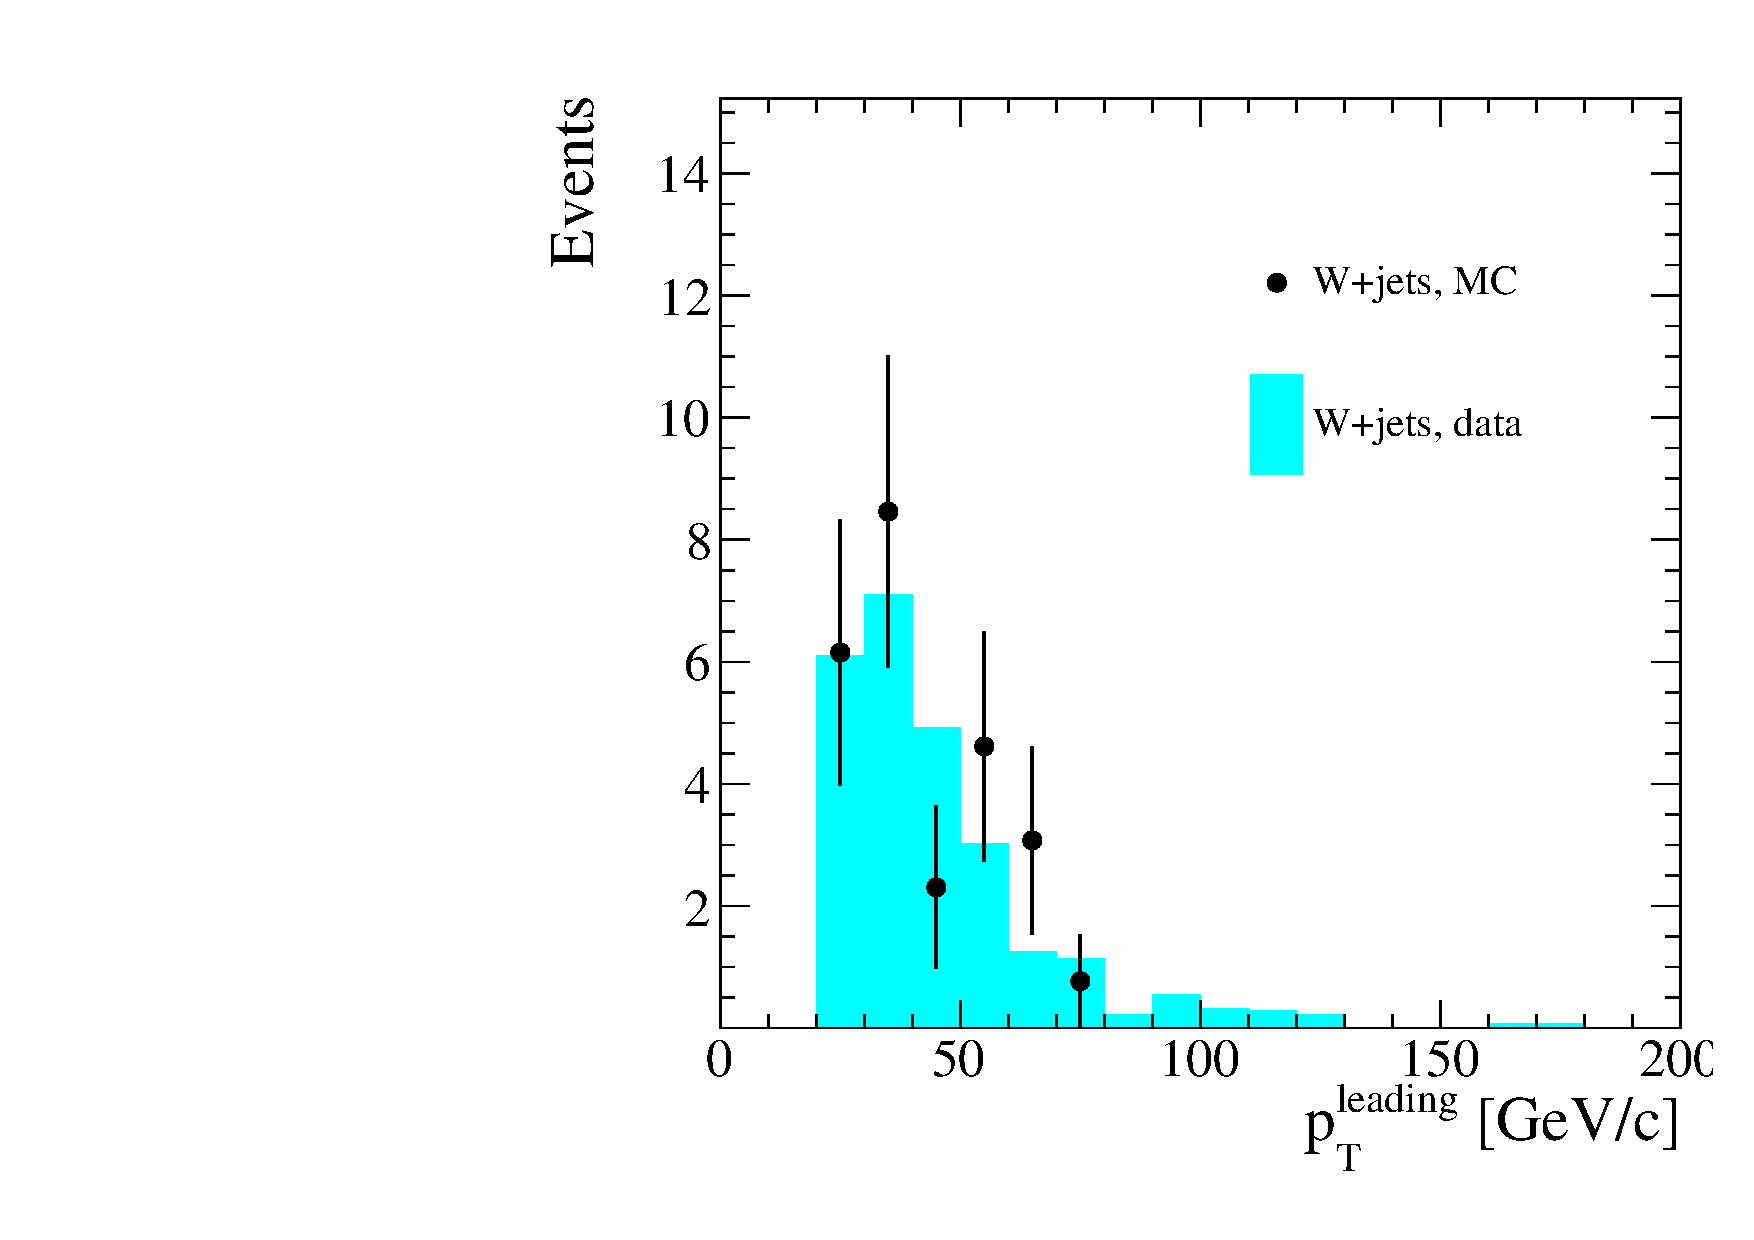
\includegraphics[width=0.45\textwidth]{figures/histo_wjets_ptmax.pdf}}
\subfigure[Trailing lepton $p_{T}$]{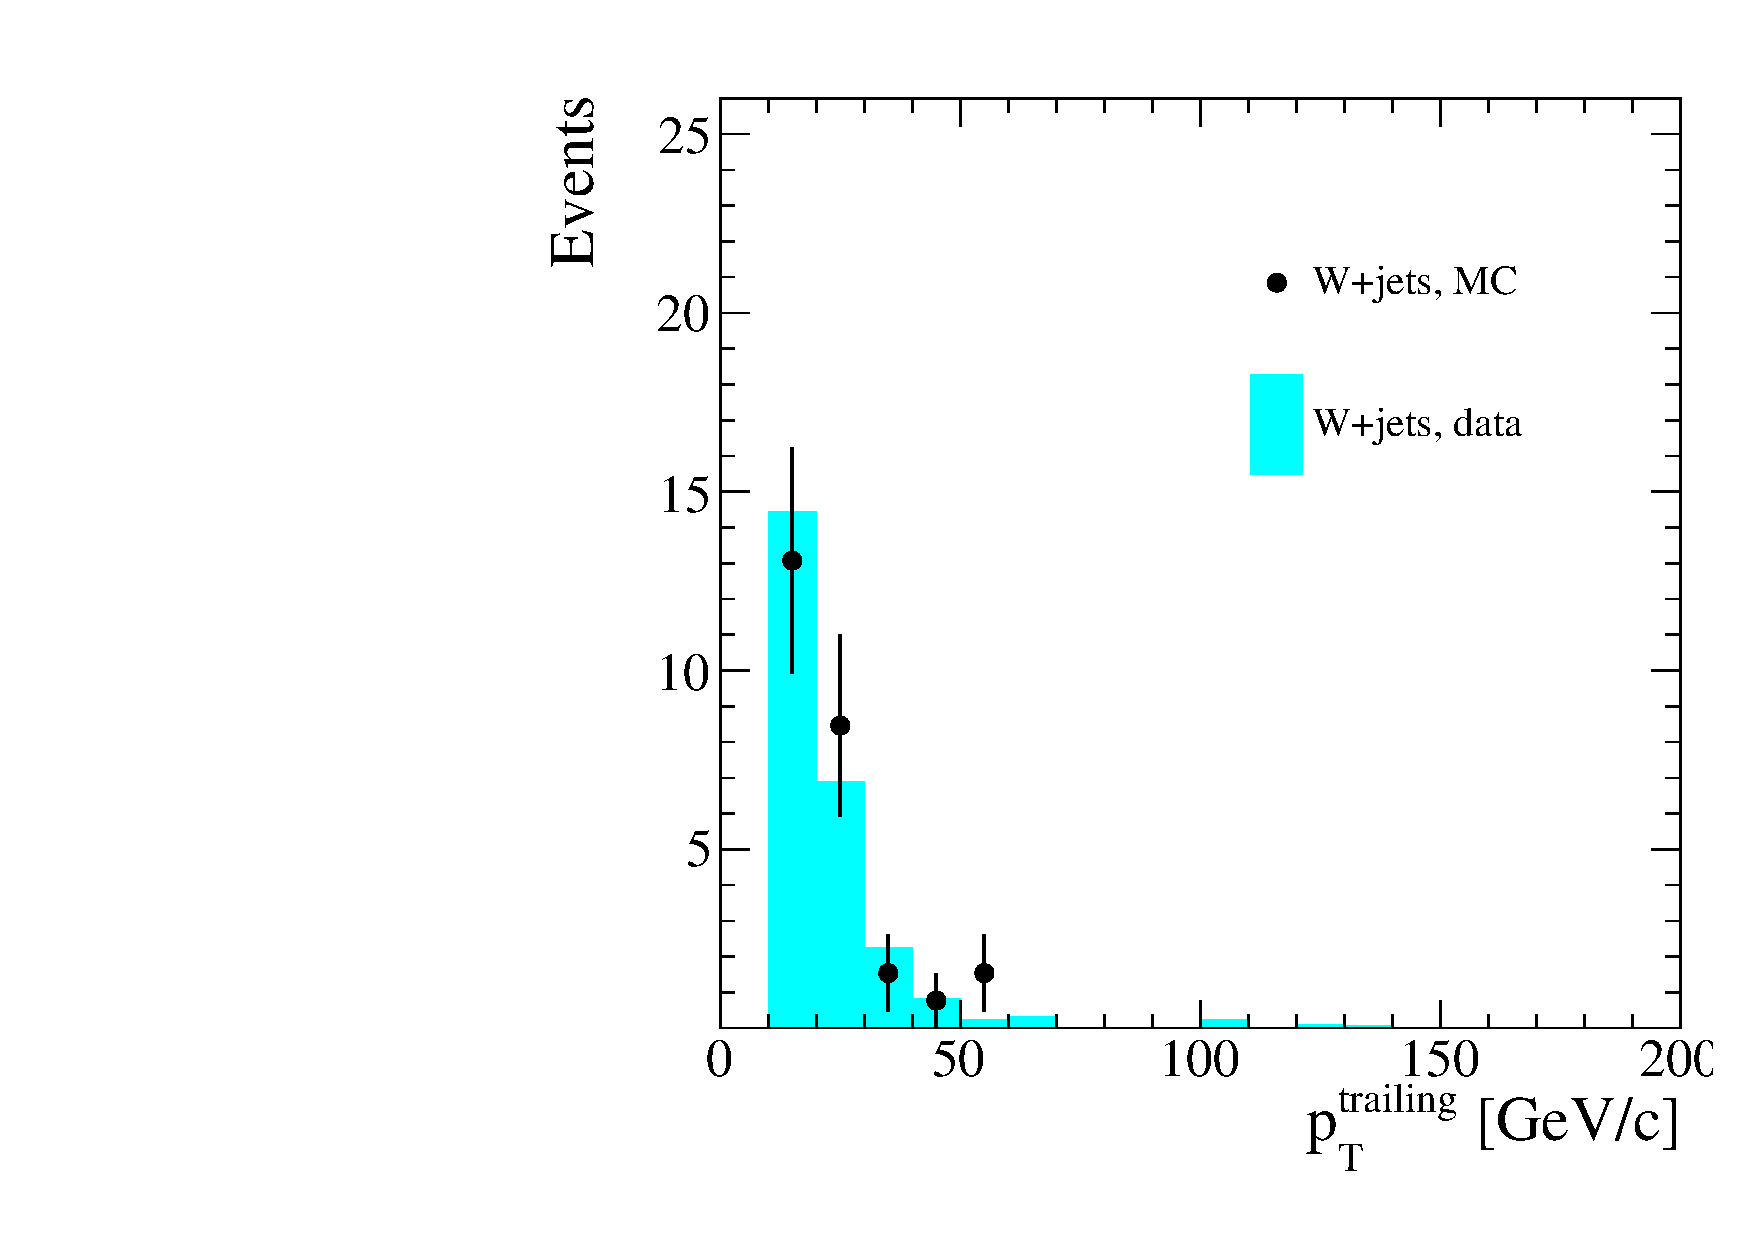
\includegraphics[width=0.45\textwidth]{figures/histo_wjets_ptmin.pdf}}
\caption{A comparison of the $p_{T}$ distribution of the leading and trailing lepton
between the fake rate method prediction and the W+Jets Pythia MC simulation prediction 
(simulation is scaled to data). }
\label{fig:FakeBkgDataDistribution_LeptonPt}
\end{center}
\end{figure}

\begin{figure}[!htbp]
\begin{center}
\subfigure[$\met$]{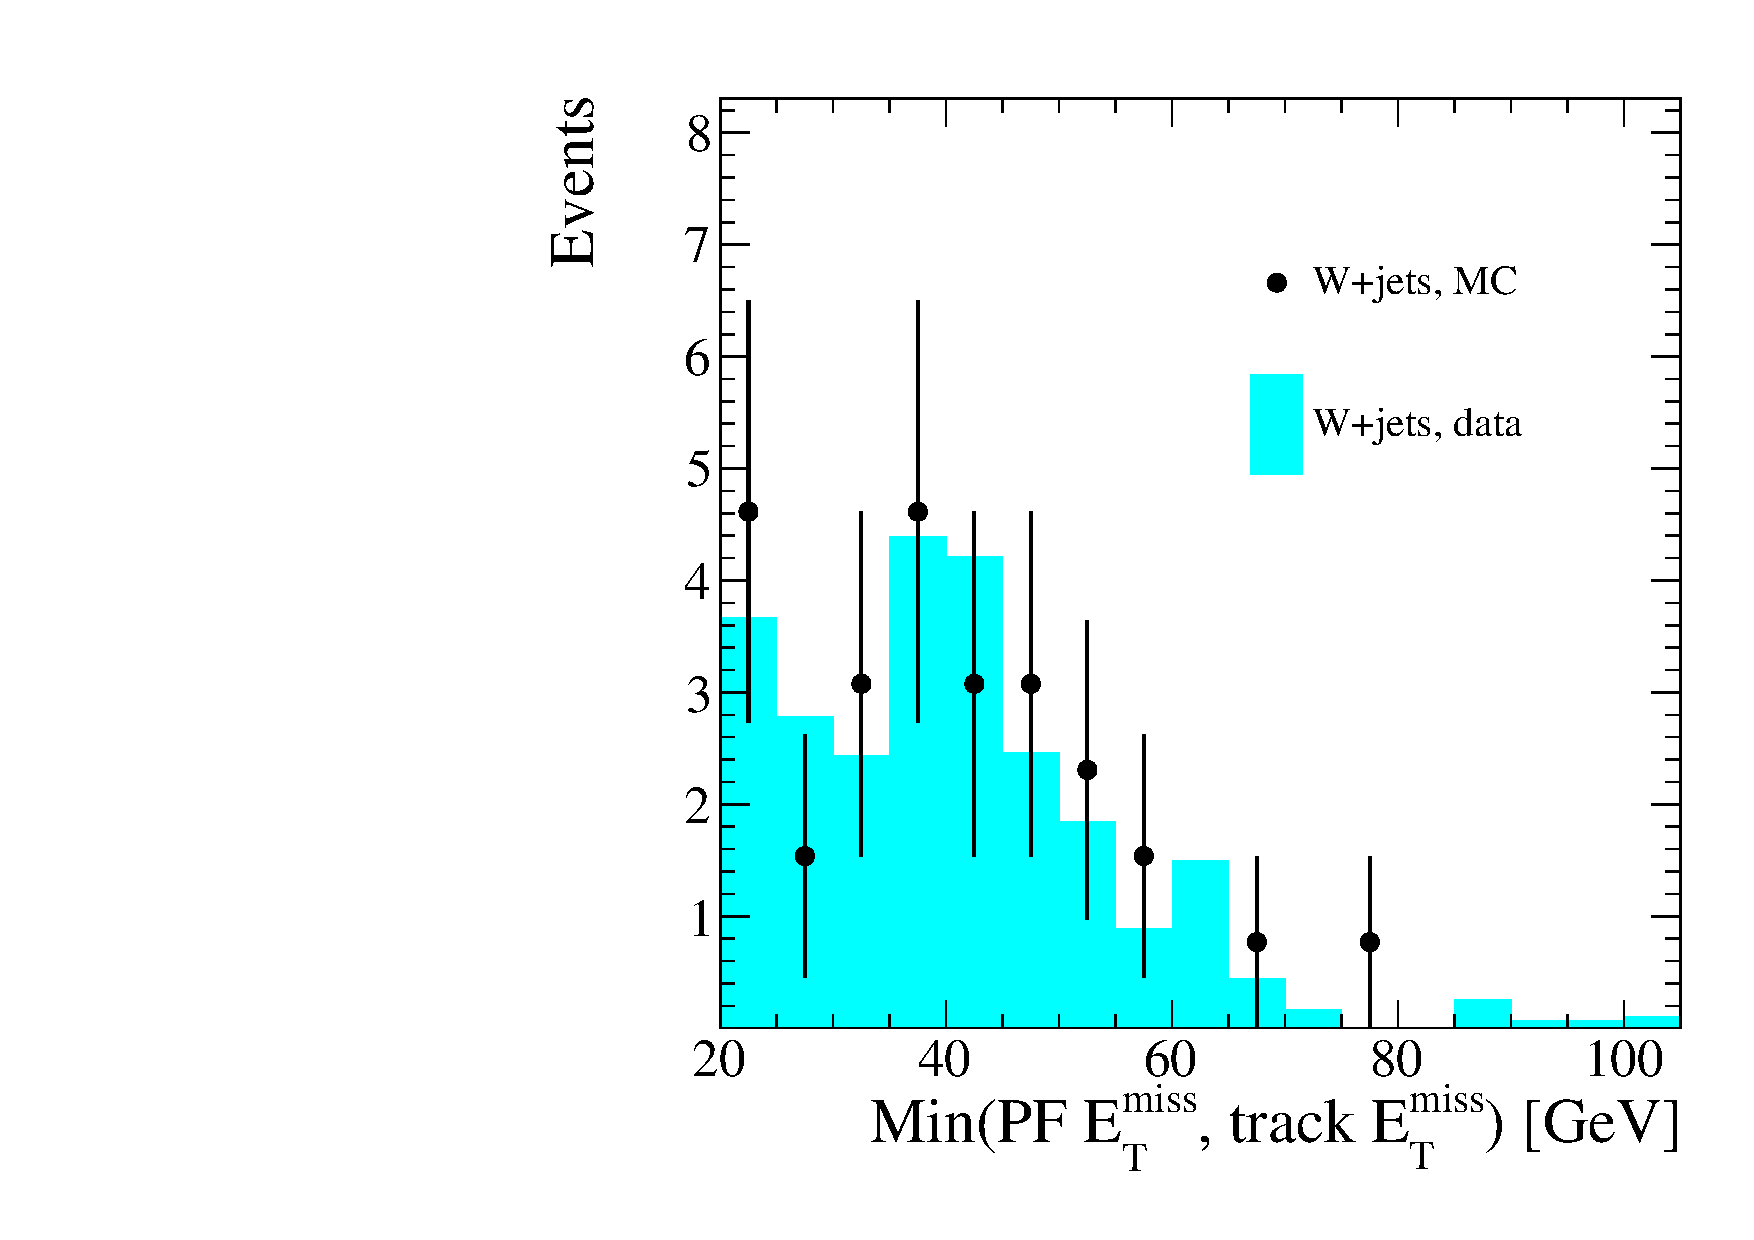
\includegraphics[width=0.45\textwidth]{figures/histo_wjets_pmet.pdf}}
\subfigure[$\Delta\phi$]{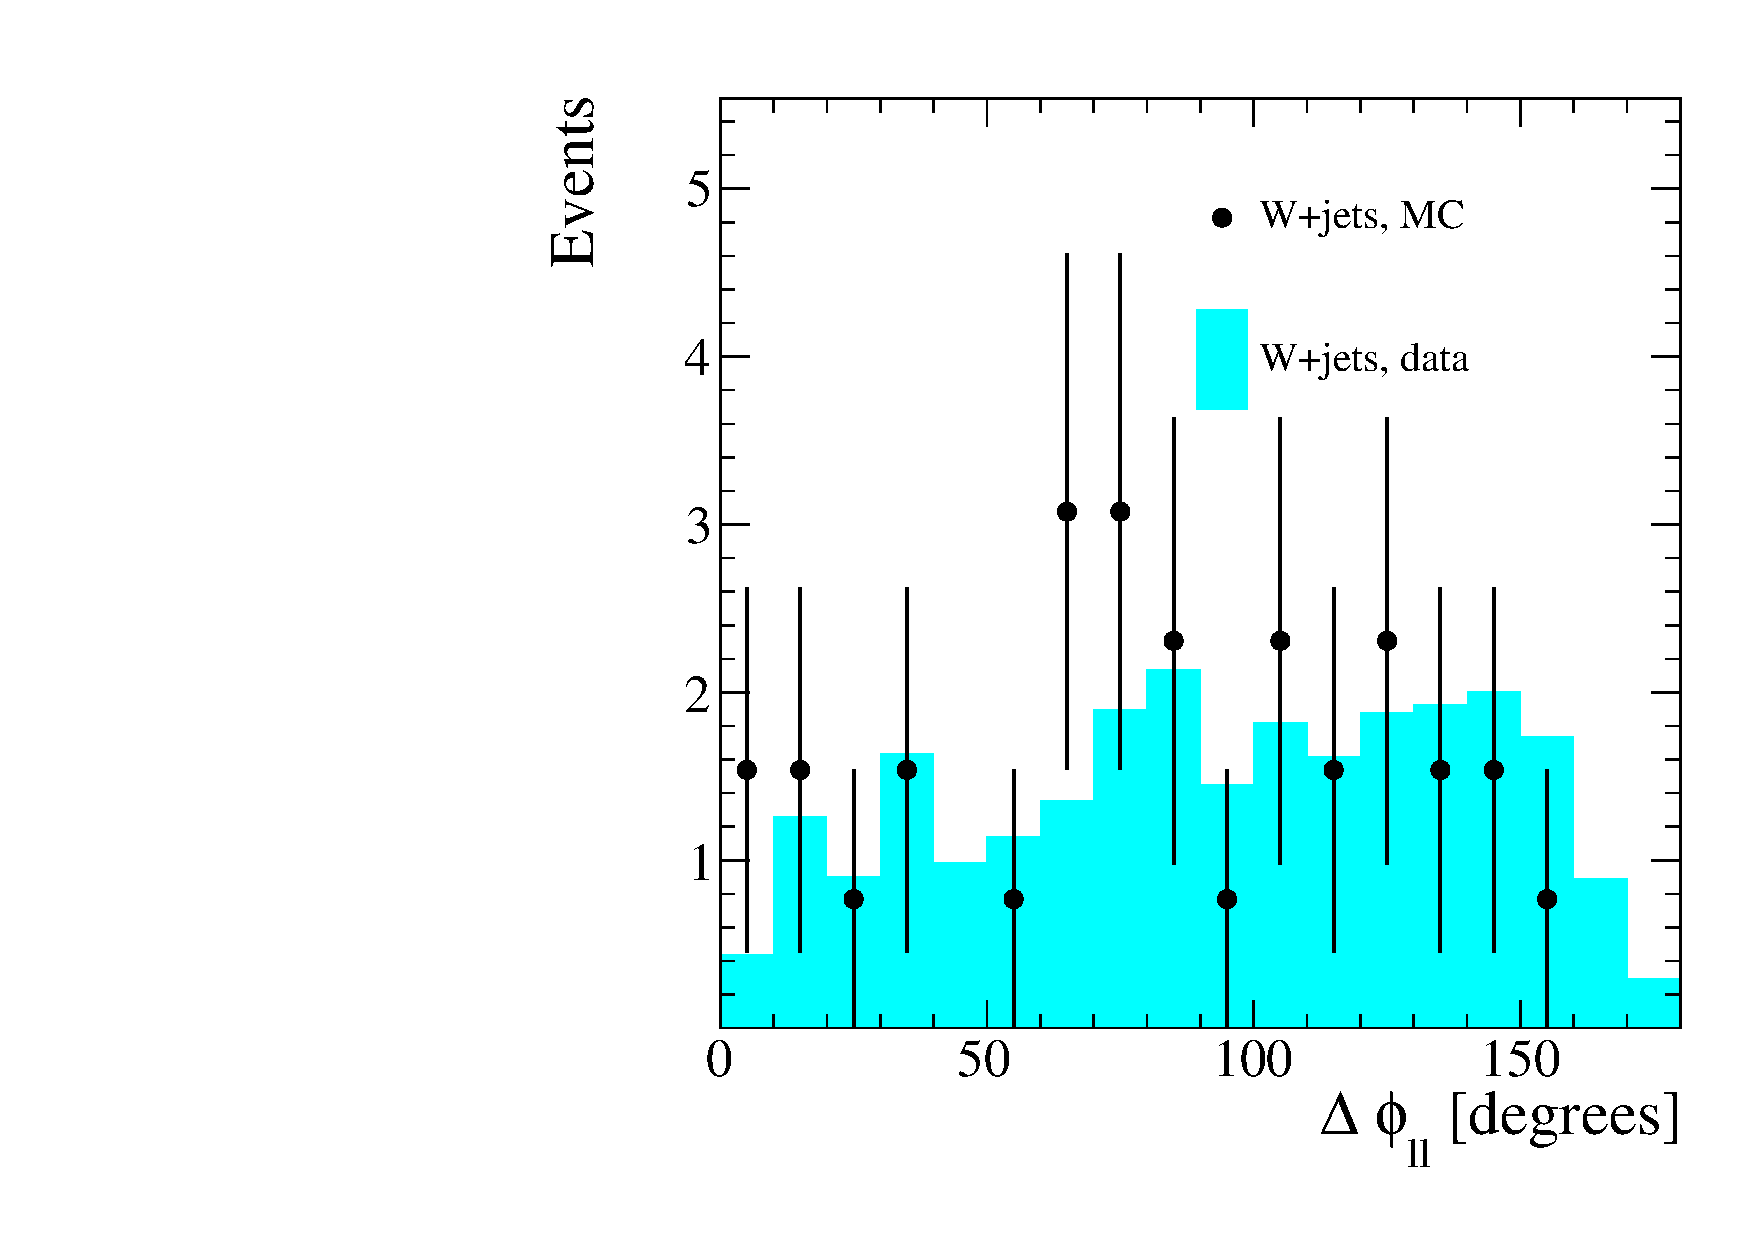
\includegraphics[width=0.45\textwidth]{figures/histo_wjets_deltaphill.pdf}}
\caption{A comparison of the distribution of the missing transverse energy, 
and the $\Delta\phi$ between the two leptons predicted using the fake rate method and the
W+Jets Pythia MC simulation (simulation is scaled to data).}
\label{fig:FakeBkgDataDistribution_MetAndDeltaPhi}
\end{center}
\end{figure}

\begin{figure}[!htbp]
\begin{center}
\subfigure[Dilepton Mass]{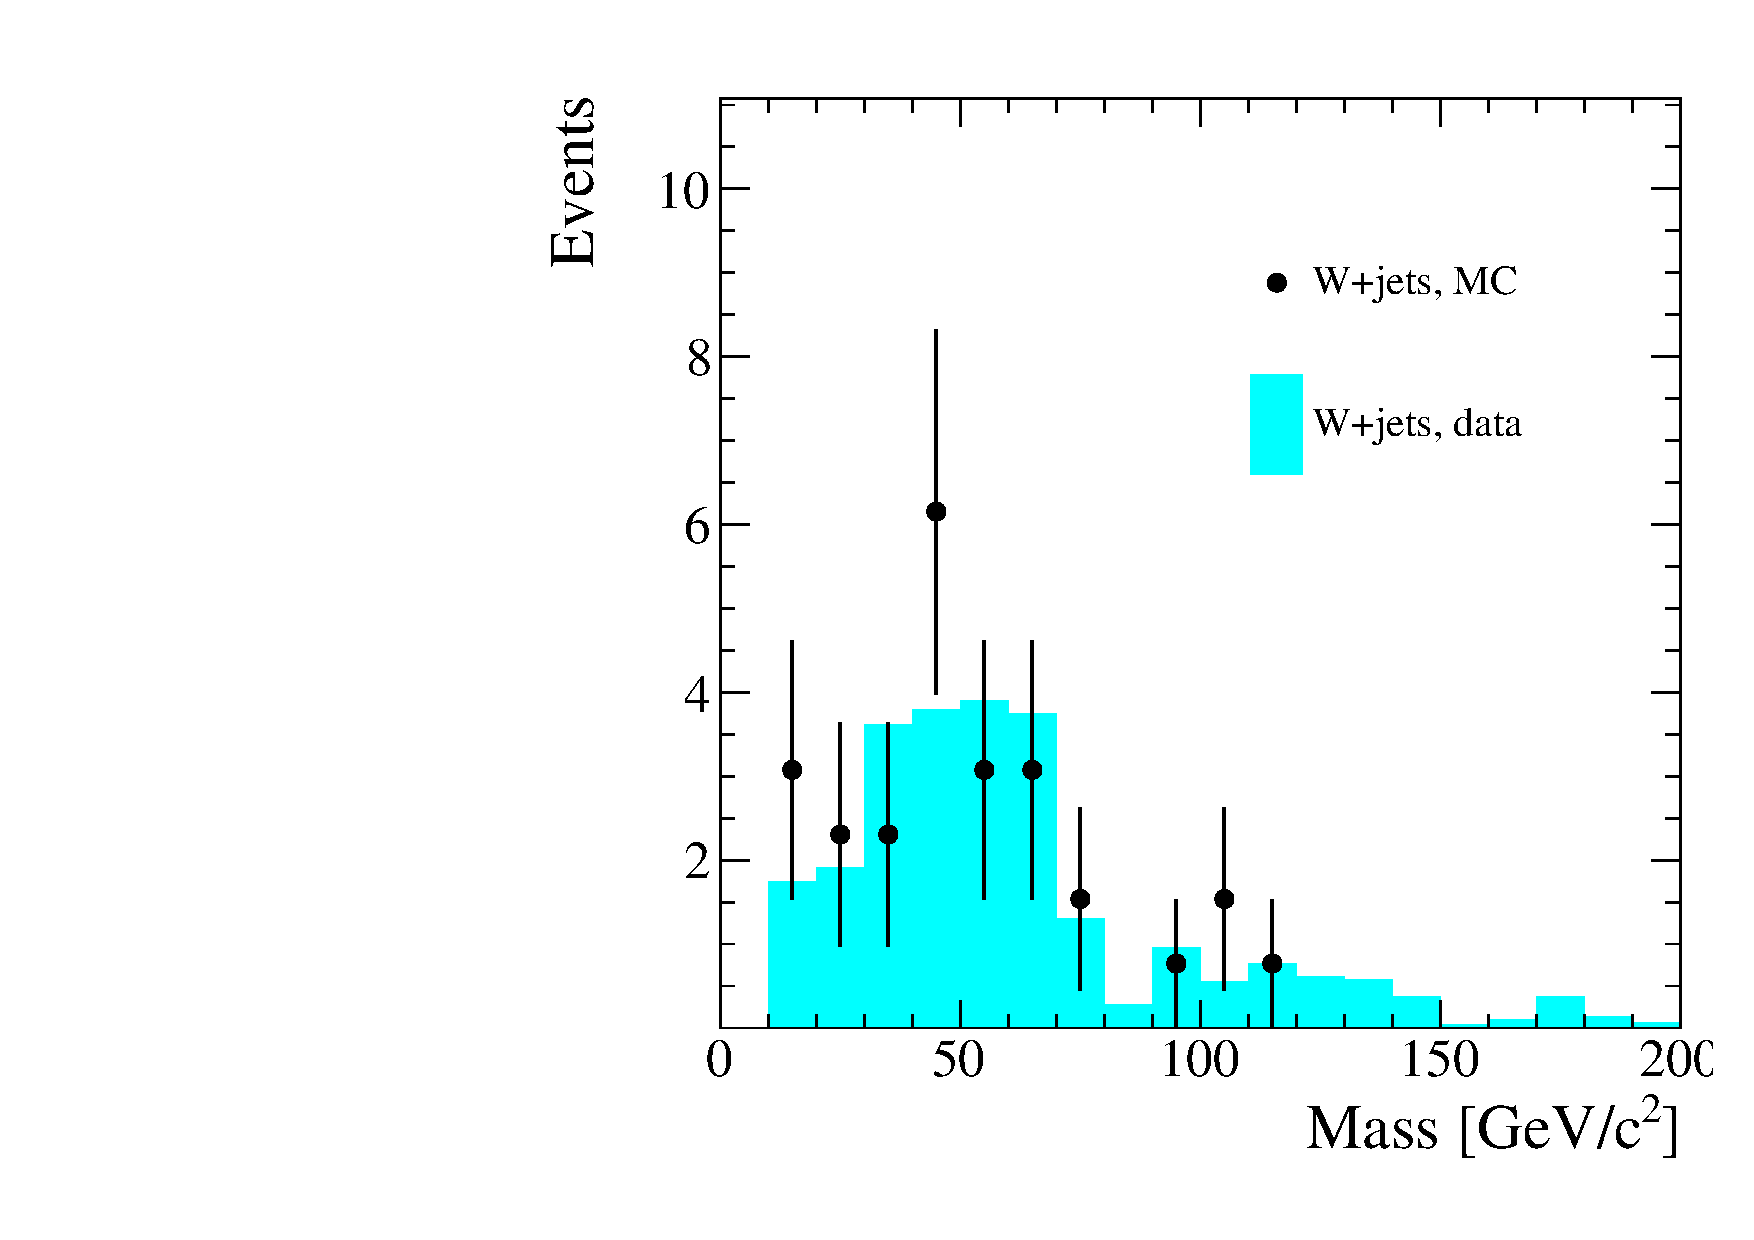
\includegraphics[width=0.45\textwidth]{figures/histo_wjets_dilmass.pdf}}
\subfigure[Higgs $M_{T}$]{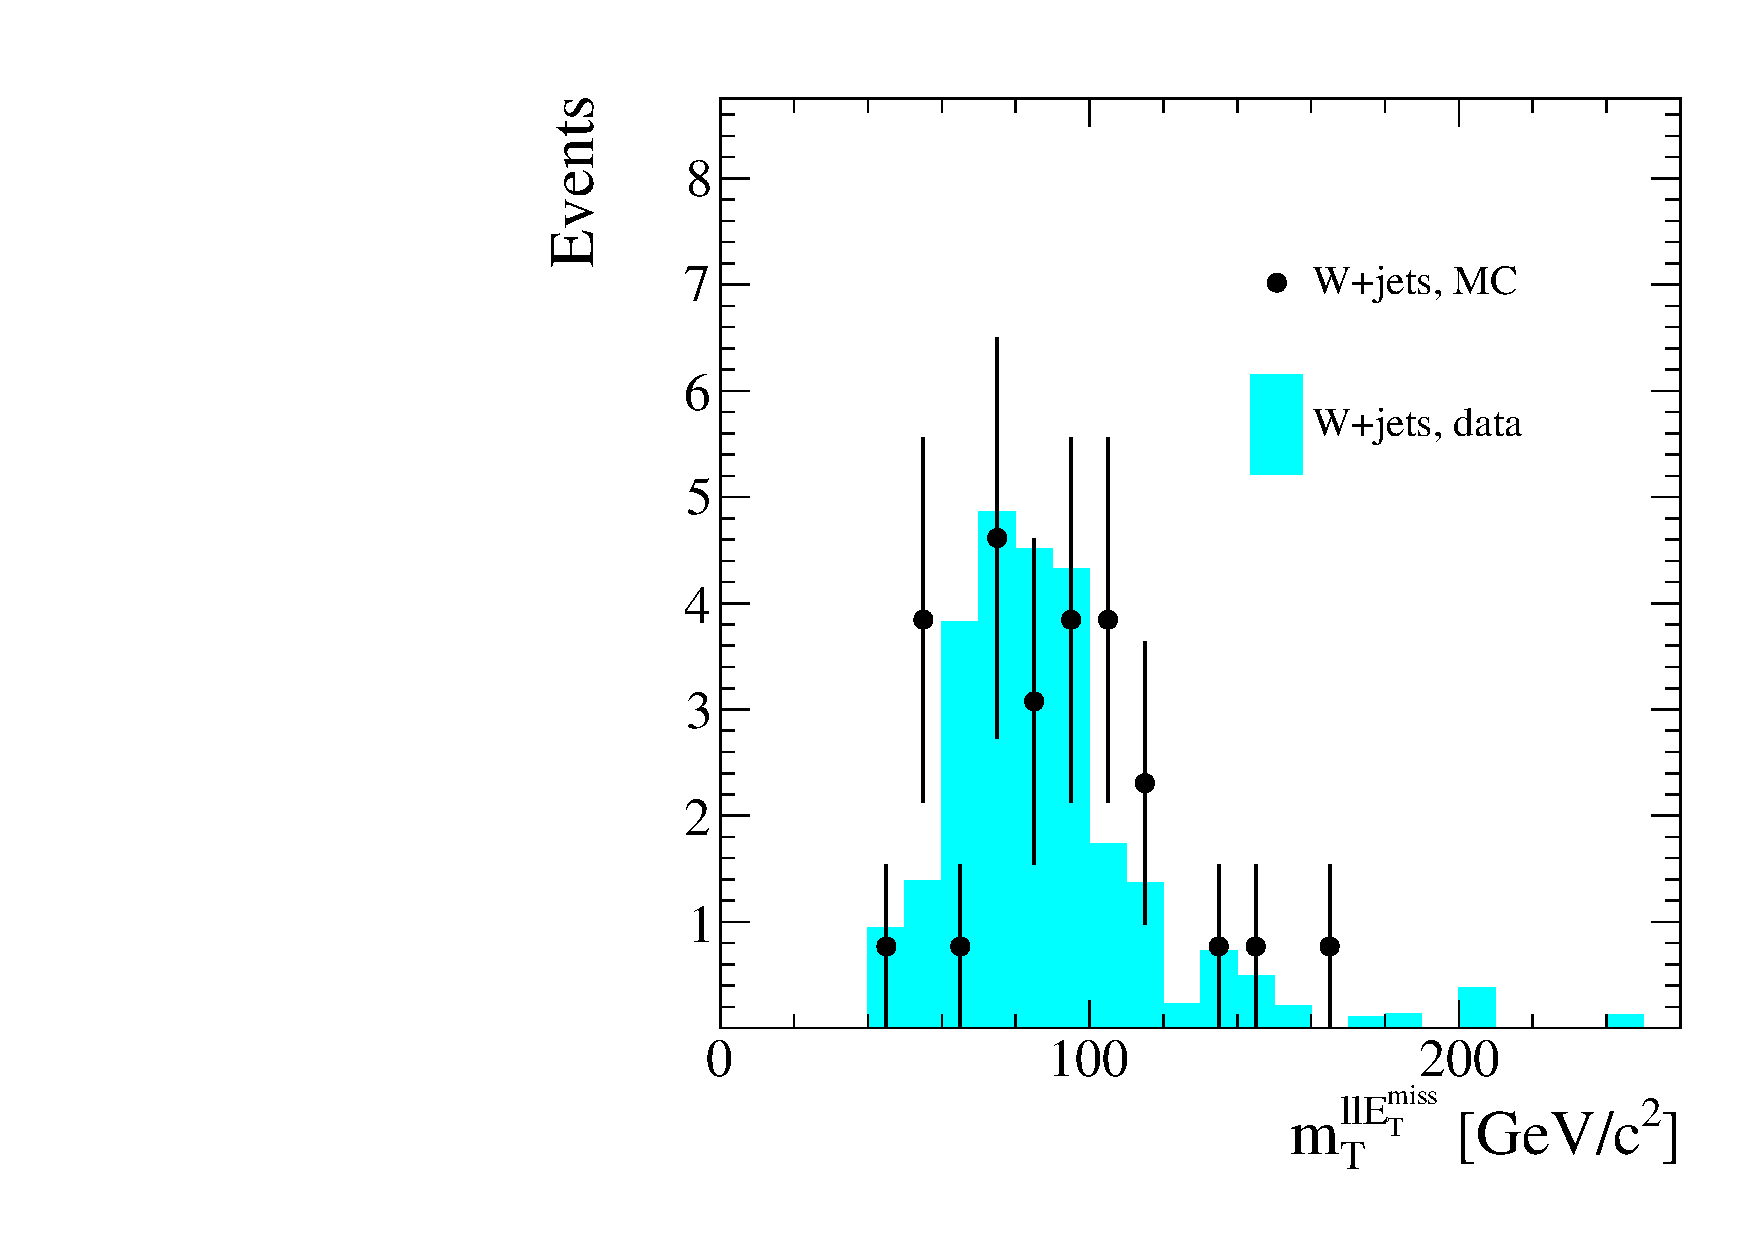
\includegraphics[width=0.45\textwidth]{figures/histo_wjets_mt.pdf}}
\caption{A comparison of the distribution of the dilepton mass and Higgs transverse mass 
predicted using the fake rate method and the W+Jets Pythia MC simulation (simulation is scaled to data).}
\label{fig:FakeBkgDataDistribution_DileptonMassAndMtHiggs}
\end{center}
\end{figure}



\subsubsection{Closure Test and Systematic Uncertainties}
\label{sec:fakerateSystematics}

The fake rate method for estimating fake lepton backgrounds, in our case
dominated by W+Jet production, crucially relies on the assumption that
fake rates can be transferred from jets in QCD events to jets in W+Jet
events. The degree to which this assumption is incorrect must be 
reflected in the systematic uncertainties of the fake lepton 
background prediction. In order to test the validity of the assumption
and to extract some quantitative measure of the systematic uncertainties,
we perform a closure test on the W+Jets Monte Carlo simulation sample by 
comparing the background yield predicted by the Monte Carlo simulation
with the yield predicted using the fake rate procedure. To be consistent,
we use the QCD Monte Carlo simulation to measure the fake rates, and then
apply them to the tight + fail sample selected in the W+Jet Monte Carlo
sample. The degree of disagreement yields a quantitative measure of the 
systematic uncertainty of the method. 

The systematic uncertainties can be factorized into two main sources. 
The first source is due to the difference in the $p_{T}$ spectrum 
of the jets in the measurement sample (QCD and Photon+Jets) compared
to the tight+fail sample (primarily W+Jets). Since we measure the 
fake rate in bins of denominator object $p_{T}$, it is clear that
for a denominator object with a given $p_{T}$, the efficiency of the
isolation cut can vary greatly depending on whether the jet producing
this denominator object has large or small $p_{T}$. The second main
source of systematic uncertainty is the composition of the fake lepton.
Due to the difference in the quark content in W+Jet events compared
to QCD events, the fractional component of fake leptons due to different 
sources or fake mechanisms may be different. Since these different sources
can typically have different fake rates (also dependent on the particular 
denominator definition that is used), the final averaged fake rate can 
be different.

To address the first source of systematic uncertainty in data, we perform the
fake rate measurement using different thresholds on the leading jet
in the event, in order to capture the degree of uncertainty in 
the jet $p_{T}$ spectrum. This systematic uncertainty is estimated to 
be $28\%$ for electrons and $31\%$ for muons, described in more detail in Appendices 
\ref{sec:FakeElectronBkgJetSpectrumSystematics} and 
\ref{sec:FakeMuonBkgJetSpectrumSystematics}. To address the second 
source of systematic uncertainty, we evaluate the agreement in the closure
test between the fake rate prediction and the simulation prediction for 
the W+Jet background. This is estimated to be $23\%$ for electrons
and $18\%$ for muons, documented in greater 
detail in Appendices \ref{sec:FakeElectronBkgClosureTest} and
\ref{sec:FakeMuonBkgClosureTest}. These two 
systematic uncertainties are added in quadrature to give a total 
systematic uncertainty of $36\%$ for electrons and $36\%$ for muons. 

Further closure tests on the fake lepton background estimate is
performed using data events with two same sign leptons. This control
sample is highly enriched in W+Jet background and can serve as an
additional cross-check of the systematic uncertainties estimated above
from Monte Carlo
simulation. Table \ref{tab:FakeLeptonBkgPrediction_SameSignSample}
summarizes the total fake lepton background estimate using the fake
rate method after the WW selection where we require that the two
leptons have the same charge instead of opposite charge. After
subtracting the non-fake background same-sign background contributions
(mostly WZ and W$\gamma$), we obtain an observed yield of $48.3\pm8.3$
and predict a yield of $48.4\pm3.6^{+11.1}_{-6.6}$. The result of this
cross-check is perfectly consistent with the uncertainties estimated
in the previous sections, demonstrating that the extrapolation
systematics estimated from the Monte Carlo simulation is applicable to
data.

\begin{table}[!htbp]
\begin{center}
\begin{tabular}{|l|c|c|}
\hline
Type           & Yield \\
\hline
Electron Fakes          &  $28.5\pm2.3^{+10.7}_{-4.2}$   \\
Muon Fakes              &  $19.9\pm2.8^{+2.9}_{-5.1}$   \\
Total                   &  $48.4\pm3.6^{+11.1}_{-6.6}$  \\
\hline
Observed same-sign events in Data        &  $68$   \\
Monte Carlo estimate of non-fake contribution (WZ \& W$\gamma)$         &  $19.7\pm1.3$\\
Fake background observed  &  $48.3\pm8.3$  \\

\hline
\end{tabular}
\caption{Summary of fake lepton background yields in the same sign sample after WW selection. }
\label{tab:FakeLeptonBkgPrediction_SameSignSample}
\end{center}
\end{table}


%% To address the second source of systematic uncertainty in data, we compare the difference in 
%% the fake rates measured in the QCD enriched selection sample and the fake rates 
%% measured in the Photon+Jet enriched selection sample. Since Photon+Jet
%% events are more similar to W+Jet events in the production mechanism,
%% one expects that fake rates measured in Photon+Jet events more closely
%% represent the fake rates in W+Jet events. 

